\section{Lecture 4 | Model Free Prediction}
Model Free Prediction is the task of estimating the value function of a given policy, 
of an unknown MDP. 

\subsection{Monte Carlo Reinforcement Learning}
Monte Carlo (MC) methods learn directly from the episodes of experience collected by
the agent, by actually interacting with the environment. MC methods only require
experience, not a model of the environment, thus requiring no knowledge of the MDP transition 
and or reward functions. MC methods learn from the complete episodes,
i.e. they dont use \emph{bootstrapping} (updating estimates based 
on other estimates). The main idea behind the MC methods is that the value
function is estimated as the mean return (over all the episodes).

\begin{note}
    MC methods can be only applied to episodic MDPs, i.e. 
    All episodes must terminate.
\end{note}

\subsubsection*{Monte Carlo Policy Evaluation}
The goal of Monte Carlo Policy Evaluation is to estimate the value function
\(v_{\pi}\) from the episodes of experience under policy \(\pi\).
Thus,
\[
    S_1, A_1, R_2, \dots, S_k  \sim \pi
\]
where \(S_k\) is the terminal state. The return \(G_t\) is the total discounted
reward from time-step \(t\).
\[
    G_t = R_{t+1} + \gamma R_{t+2} + \dots + \gamma^{T-1}R_T
\]
where \(T\) is the final time-step. The value function \(v_{\pi}(s)\) is the
expected return when starting in \(s\) and following \(\pi\).
\[
    v_{\pi}(s) = \mathbb{E}_{\pi}[G_t | S_t = s]
\]
The value function \(v_{\pi}(s)\) is estimated as the mean return (over all the
episodes). Thus, the MC policy evaluation uses empirical mean return instead of the
expected return.

\subsubsection{First-Visit MC Policy Evaluation}
The first-visit MC policy evaluation is the simplest MC method. It estimates
the value function \(v_{\pi}(s)\) as the average of the returns following first
visits to \(s\). Thus, it averages the returns following all the first visits to
\(s\).
The algorithm for the first-visit MC policy evaluation is given as, with the 
pseudo-code in \autoref{alg:first_visit_mc}.
\begin{enumerate}
    \item For each state \(s\), maintain two variables:
    \begin{itemize}
        \item \(N(s)\) - the number of times that \(s\) has been visited.
        \item \(S(s)\) - the sum of the returns that have followed first visits to \(s\).
    \end{itemize}
    \item For each episode \(E = S_1, A_1, R_2, \dots, S_k\), for each state \(S_t\) 
    in the episode:
    \begin{itemize}
        \item \(N(S_t) \leftarrow N(S_t) + 1\)
        \item \(S(S_t) \leftarrow S(S_t) + G_t\)
    \end{itemize}
    \item For each state \(s\), estimate \(v_{\pi}(s)\) as the average return:
    \[
        V(s) = \frac{S(s)}{N(s)}
    \]
    where \(V(s)\) is the estimate of \(v_{\pi}(s)\).
\end{enumerate}
By the law of large numbers, \(V(s) \to v_{\pi}(s)\) as \(N(s) \to \infty\). 

\begin{algorithm}[H]
    \caption{First Visit Monte Carlo Policy Evaluation}
    \label{alg:first_visit_mc}
    \begin{algorithmic}[1]
        \For{each state $s$}
            \State Initialize $N(s)$ - the number of times that $s$ has been visited.
            \State Initialize $S(s)$ - the sum of the returns that have followed first visits to $s$.
        \EndFor
        \For{each episode $E = S_1, A_1, R_2, \dots, S_k$}
            \For{each state $S_t$ in the episode}
                \State $N(S_t) \leftarrow N(S_t) + 1$
                \State $S(S_t) \leftarrow S(S_t) + G_t$
            \EndFor
        \EndFor
        \For{each state $s$}
            \State Estimate $v_{\pi}(s)$ as the average return:
            \[
                V(s) = \frac{S(s)}{N(s)}
            \]
        \EndFor
    \end{algorithmic}
\end{algorithm}

\subsubsection{Every-Visit MC Policy Evaluation}
The every-visit MC policy evaluation is similar to the first-visit MC policy, with
the exception that it averages the returns following all the visits to \(s\). Thus,
\begin{enumerate}
    \item For each state \(s\), maintain two variables:
    \begin{itemize}
        \item \(N(s)\) - the number of times that \(s\) has been visited.
        \item \(S(s)\) - the sum of the returns that have followed visits to \(s\).
    \end{itemize}
    \item For each episode \(E = S_1, A_1, R_2, \dots, S_k\), for each state \(S_t\) 
    in the episode:
    \begin{itemize}
        \item \(N(S_t) \leftarrow N(S_t) + 1\)
        \item \(S(S_t) \leftarrow S(S_t) + G_t\)
    \end{itemize}
    \item For each state \(s\), estimate \(v_{\pi}(s)\) as the average return:
    \[
        V(s) = \frac{S(s)}{N(s)}
    \]
    where \(V(s)\) is the estimate of \(v_{\pi}(s)\).
\end{enumerate}
By the law of large numbers, \(V(s) \to v_{\pi}(s)\) as \(N(s) \to \infty\). The pseudo-code
for the every-visit MC policy evaluation is given in \autoref{alg:every_visit_mc}.
\begin{algorithm}[H]
    \caption{Every Visit Monte Carlo Policy Evaluation}
    \label{alg:every_visit_mc}
    \begin{algorithmic}[1]
        \For{each state $s$}
            \State Initialize $N(s)$ - the number of times that $s$ has been visited.
            \State Initialize $S(s)$ - the sum of the returns that have followed visits to $s$.
        \EndFor
        \For{each episode $E = S_1, A_1, R_2, \dots, S_k$}
            \For{each state $S_t$ in the episode}
                \State $N(S_t) \leftarrow N(S_t) + 1$
                \State $S(S_t) \leftarrow S(S_t) + G_t$
            \EndFor
        \EndFor
        \For{each state $s$}
            \State Estimate $v_{\pi}(s)$ as the average return:
            \[
                V(s) = \frac{S(s)}{N(s)}
            \]
        \EndFor
    \end{algorithmic}
\end{algorithm}

\subsubsection*{Incremental Mean}
The incremental mean is a method to compute the mean of a sequence of numbers.
The mean \(\mu_1, \mu_2, \dots, \mu_n\) of a sequence of numbers \(x_1, x_2, \dots, x_n\)
is given as,
\[
    \begin{aligned}
        \mu_k &= \frac{1}{k}\sum_{j=1}^{k}x_j \\
        &= \frac{1}{k}(x_k + \sum_{j=1}^{k-1}x_j) \\
        &= \frac{1}{k}(x_k + (k-1)\mu_{k-1}) \\
        &= \mu_{k-1} + \frac{1}{k}(x_k - \mu_{k-1})      
    \end{aligned}
\] 
Thus, the mean of the sequence can be computed incrementally, using the previous
mean and the current element of the sequence. All the main algorithms that we will see in
this lecture follow this incremental update idea. That is to update the mean (value function)
by pushing the current estimate to the previous estimate using the error in the current
estimate and the actual value obtained.

\subsubsection{Incremental Monte Carlo Updates}
The estimate of the value function \(V(s)\) is updated incrementally after each episode
\(E = S_1, A_1, \\R_2, \dots, S_k\). Thus, for each state \(S_t\) with return \(G_t\),
\[
    \begin{aligned}
        N(S_t) &\leftarrow N(S_t) + 1 \\
        V(S_t) &\leftarrow V(S_t) + \frac{1}{N(S_t)}\left( 
            G_t - V(S_t)
         \right) 
    \end{aligned}
\]
where \(N(S_t)\) is the number of times that \(S_t\) has been visited and \(V(S_t)\)
is the current estimate of \(v_{\pi}(S_t)\). In non-stationary problems, the step size
\(\alpha\) can be used to control the rate of convergence of the value function, rather
than keeping the track of the number of visits to each state. This is done on the intuition
that the more recent returns are more important than the past returns, as the current
dynamics might differ from the past dynamics.
Thus, the update rule becomes,
\[
    \begin{aligned}
        V(S_t) &\leftarrow V(S_t) + \alpha\left( 
            G_t - V(S_t)
         \right) 
    \end{aligned}
\]

\subsection{Temporal Difference Learning}
Similar to the MC methods, the Temporal Difference (TD) methods learn directly from the
episodes of experience collected by the agent, by actually interacting with the environment.
TD methods only require experience, not a model of the environment, thus requiring no knowledge
of the MDP transition and or reward functions. TD methods learn from the incomplete episodes,
i.e. they use \emph{bootstrapping} (updating estimates based on other estimates). The main
idea behind the TD updates the guess towards the guess.

\subsubsection*{MC vs TD}
Goal of both MC and TD is to estimate \(v_{\pi}(s)\) from experience under policy \(\pi\).
In every-visit MC:
\[
    V(S_t) \leftarrow V(S_t) + \alpha\left( 
        G_t - V(S_t)
     \right)      
\]
While in the simplest TD method, TD(0), the update value is tageted towards the estimated
return \(R_{t+1} + \gamma V(S_{t+1})\).
\[
    V(S_t) \leftarrow V(S_t) + \alpha\left( 
        \underset{\text{TD Target} }{\underbrace{R_{t+1} + \gamma V(S_{t+1})}}
        - V(S_t)
     \right)
\]
The TD error is defined as,
\[
    \delta_t = R_{t+1} + \gamma V(S_{t+1}) - V(S_t)
\]

\subsubsection{Advantages and Disadvantages of MC vs TD}
\begin{itemize}
    \item  TD can learn before knowing the final outcome
    \begin{itemize}
        \item TD can learn online after every step
        \item MC must wait until the end of the episode
    \end{itemize}
    \item TD can learn without the final outcome
    \begin{itemize}
        \item TD can learn from incomplete sequences
        \item MC can only learn from complete sequences
        \item TD works in continuing (non-terminating) environments
        \item MC only works for episodic (terminating) environments
    \end{itemize}
\end{itemize}

\subsubsection*{Bias/Variance Trade-off}
The return \(G_t = R_{t+1} + \gamma R_{t+2} + \dots + \gamma^{T-1}R_T\) is an \emph{unbiased}
estimate of \(v_{\pi}(S_t)\). Thus, \(\mathbb{E}[G_t | S_t = s] = v_{\pi}(s)\). Moreover,
the True TD Target \(R_{t+1} + \gamma v_\pi (S_{t+1})\) is also an unbiased estimate of
\(v_{\pi}(S_t)\). 
But, the TD Target \(R_{t+1} + \gamma V(S_{t+1})\) is a \emph{biased} estimate of \(v_{\pi}(S_t)\).

One advantage that TD has in comparison to MC is that the TD target has lower variance
compared to the return. This can be seen from the fact that the return depends 
on many random actions, transitions and rewards, while the TD target depends on only one
random action, transition and reward.

In summary:
\begin{itemize}
    \item MC has \emph{high variance}, zero bias
    \begin{itemize}
        \item Good convergence properties
        \item Even with function approximation
        \item Not very sensitive to initial value
    \end{itemize}
    \item TD has \emph{low variance}, some bias
    \begin{itemize}
        \item Usually converges faster than MC
        \item TD(0) converges to \(v_{\pi}\)
        \item may not converge with function approximation
        \item Sensitive to initial value
    \end{itemize}
\end{itemize}

\subsubsection{Batch MC and TD}
Both MC and TD methods converge to \(v_{\pi}\) as the number of episodes \(N \to \infty\). 
But what if we only have a batch of finite experiences:
\[
    \begin{aligned}
        & s^1_1, a^1_1, r^1_2, \dots, s^1_{T_1} \\
        & s^2_1, a^2_1, r^2_2, \dots, s^2_{T_2} \\
        &\vdots \quad \dots  \quad \vdots \\
        & s^K_1, a^K_1, r^K_2, \dots, s^K_{T_K} \\
    \end{aligned}
\]
Thus, we repedeatdly sample episode \(k \in [1,K]\) and apply MC or TD(0) to
episode \(k\).

\begin{example}[AB Example]
    Two states \(A\) and \(B\); no discounting; with 8 episodes of experience as:
    \begin{figure}[H]
        \begin{minipage}{0.5\textwidth}
          \[
            \begin{aligned}
                A, & 0, B, 0 \\
                B, & 1\\ 
                B, & 1\\        
                B, & 1\\        
                B, & 1\\        
                B, & 1\\        
                B, & 1\\        
                B, & 0\\        
            \end{aligned}
          \]
        \end{minipage}%
        \begin{minipage}{0.5\textwidth}
          % Your image goes here
          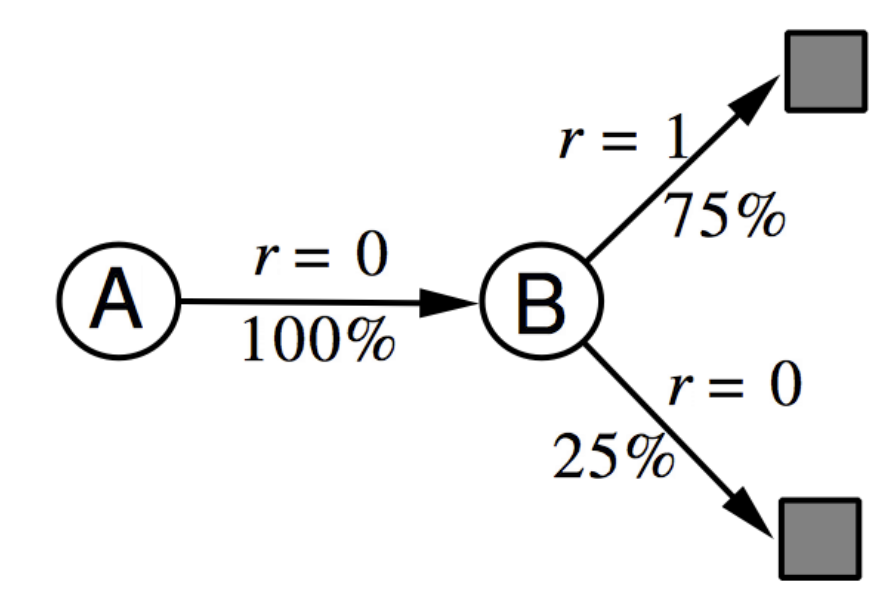
\includegraphics[width=\textwidth]{figures/ab-ex.png}
          \caption{AB Example}
            \label{fig:ab_ex}
        \end{minipage}
      \end{figure}
      What is \(V(A)\) and \(V(B)\) ?

      Solution: \(V(B) = 0.75\), while \(V(A) = 0.75 \text{ and } 0\), and are the soltuions
      using TD and MC respectively.
\end{example}

\subsubsection*{Certainty Equivalence}
\begin{itemize}
    \item MC Converges to the solution with minimum mean squared error. Thus it best fits to 
    the observered returns.
    \[
        \sum_{k=1}^{K}\sum_{t=1}^{T_k}(G_t^k - V(S_t^k))^2 
    \]
    In the AB example, the MC solution is \(V(A) = 0\).
    \item TD Converges to the solution of maximum likelihood Markov model. Thus it gives
    the solution to the MDP \( \langle \mathcal{S}, \mathcal{A}, \mathcal{P},
     \mathcal{R}, \gamma \rangle\)  that best fits the data.
     \[
        \begin{aligned}
            \hat{\mathcal{P}}_{ss'}^a &= \frac{1}{N(s,a)}\sum_{k=1}^{K}\sum_{t=1}^{T_k}
            \bm{1}(s_t^k, a_t^k, s_{t+1}^k = s, a, s') \\
            \hat{\mathcal{R}}_{s}^a &= \frac{1}{N(s,a)}\sum_{k=1}^{K}\sum_{t=1}^{T_k}
            \bm{1}(s_t^k, a_t^k = s, a)r_{t+1}^k
        \end{aligned}
     \]
     In the AB example, the TD solution is \(V(A) = 0.75\).
\end{itemize}

\subsection{Unified View of Reinforcement Learning}
\begin{figure}[H]
    \begin{minipage}{0.5\textwidth}
        Monte Carlo Backup:
      \[
        V(S_t) \leftarrow V(S_t) + \alpha\left( 
            G_t - V(S_t)
         \right)
      \]
    \end{minipage}%
    \begin{minipage}{0.5\textwidth}
      % Your image goes here
      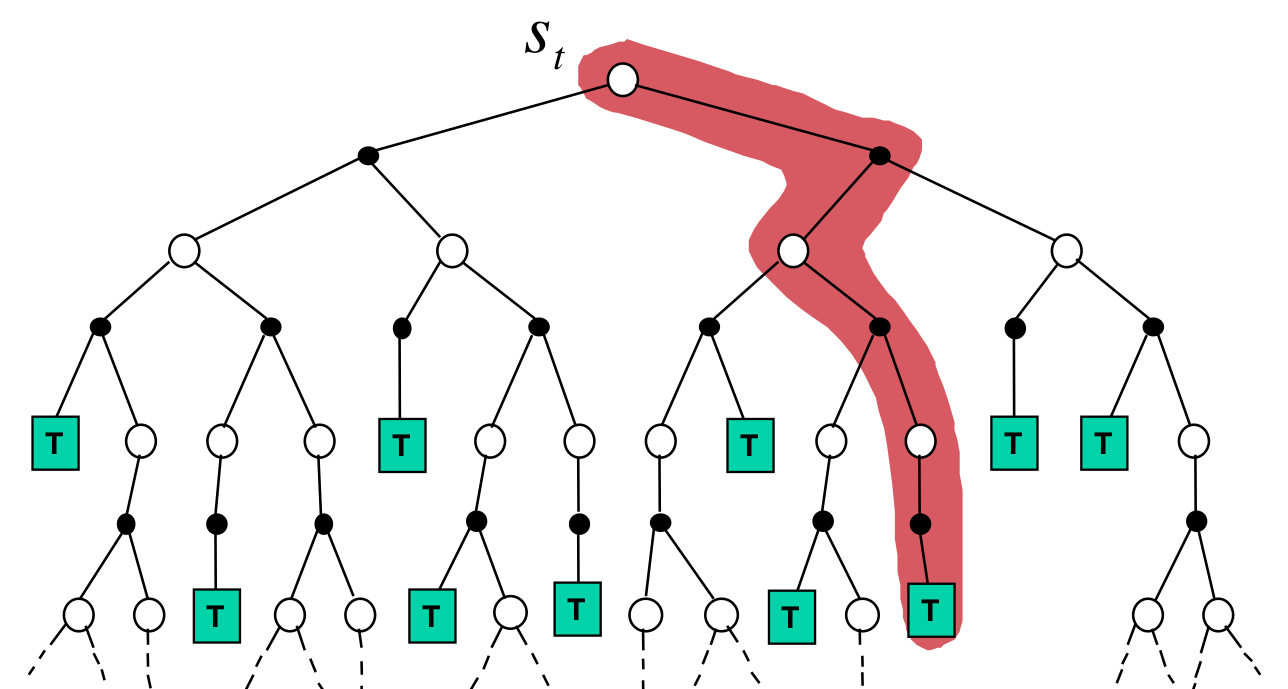
\includegraphics[width=\textwidth]{figures/uni-mc.png}
      \caption{Tree Backup of Monte Carlo Learning}
        \label{fig:uni-mc}
    \end{minipage}
\end{figure}

\begin{figure}[H]
    \begin{minipage}{0.5\textwidth}
        TD Backup:
      \[
        V(S_t) \leftarrow V(S_t) + \alpha\left( 
            R_{t+1} + \gamma V(S_{t+1}) - V(S_t)
         \right)
      \]
    \end{minipage}%
    \begin{minipage}{0.5\textwidth}
      % Your image goes here
      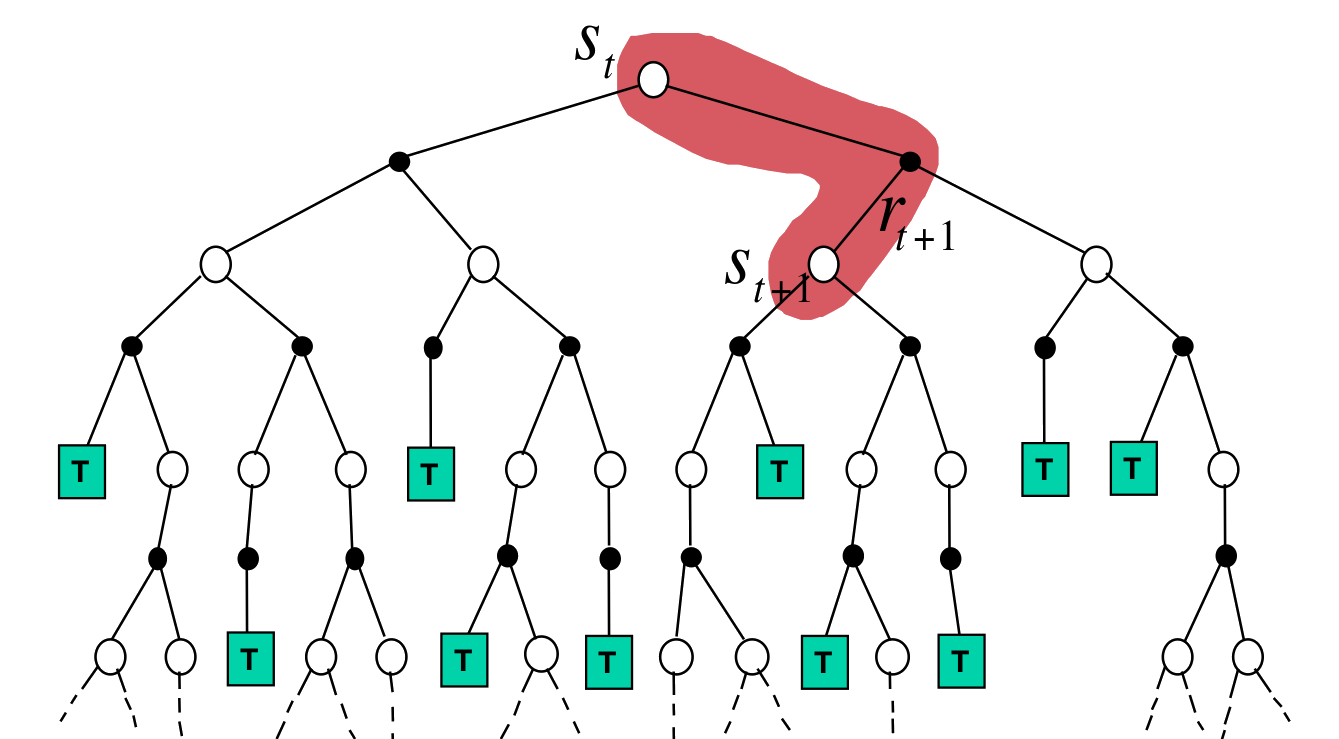
\includegraphics[width=\textwidth]{figures/uni-td.png}
      \caption{Tree Backup of TD Learning}
        \label{fig:uni-td}
    \end{minipage}
\end{figure}
%Dynamics Programming Backup:
\begin{figure}[H]
    \begin{minipage}{0.5\textwidth}
        Dynamic Programming Backup:
      \[
        V(S_t) \leftarrow \mathbb{E}_\pi \left[ 
            R_{t+1} + \gamma V(S_{t+1})
         \right]
      \]
    \end{minipage}%
    \begin{minipage}{0.5\textwidth}
      % Your image goes here
      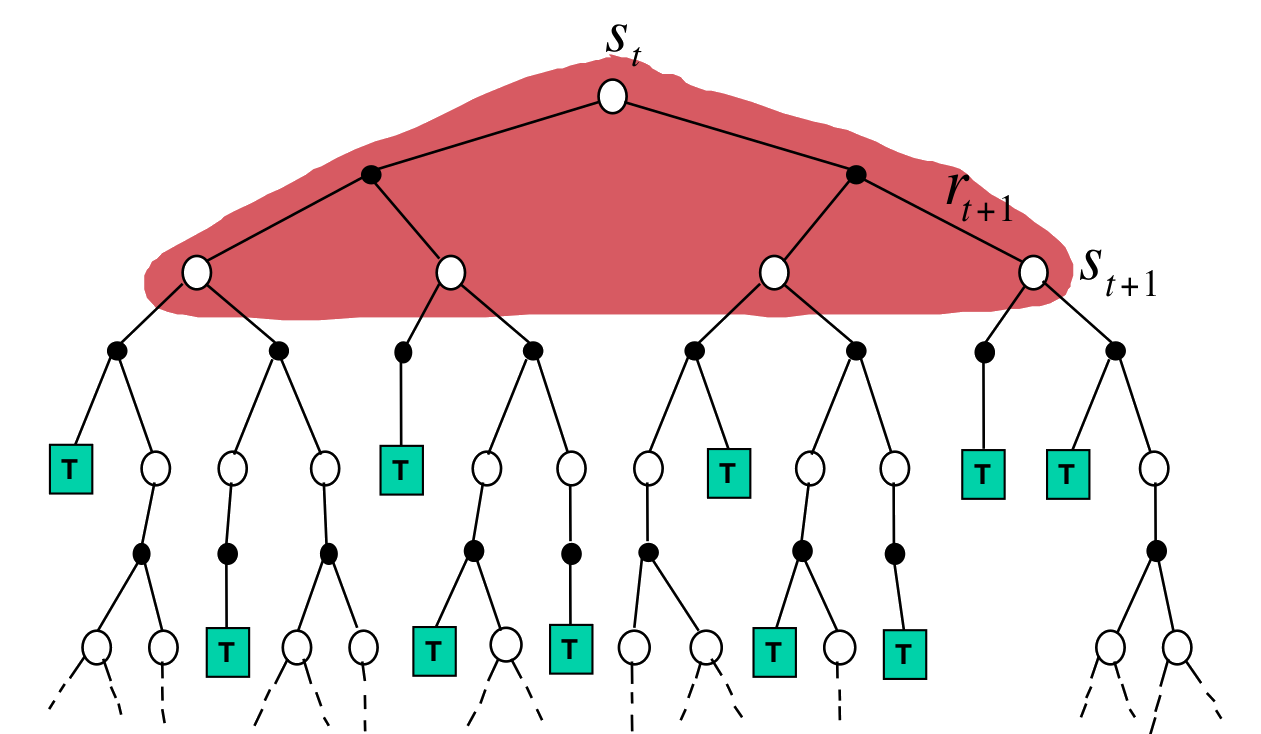
\includegraphics[width=\textwidth]{figures/uni-dp.png}
      \caption{Tree Backup of Dynamic Programming}
        \label{fig:uni-dp}
    \end{minipage}
\end{figure}

\subsubsection*{Bootstrapping and Sampling}
\begin{itemize}
    \item Bootstrapping: Update involves an estimate/guess
    \begin{itemize}
        \item MC does not bootstrap
        \item DP bootstraps
        \item TD bootstraps
    \end{itemize}
    \item Sampling: Update involves a sample of real experience or samples and expectation
    \begin{itemize}
        \item MC samples
        \item DP does not sample
        \item TD samples
    \end{itemize}
\end{itemize}

\begin{figure}[H]
    \centering
    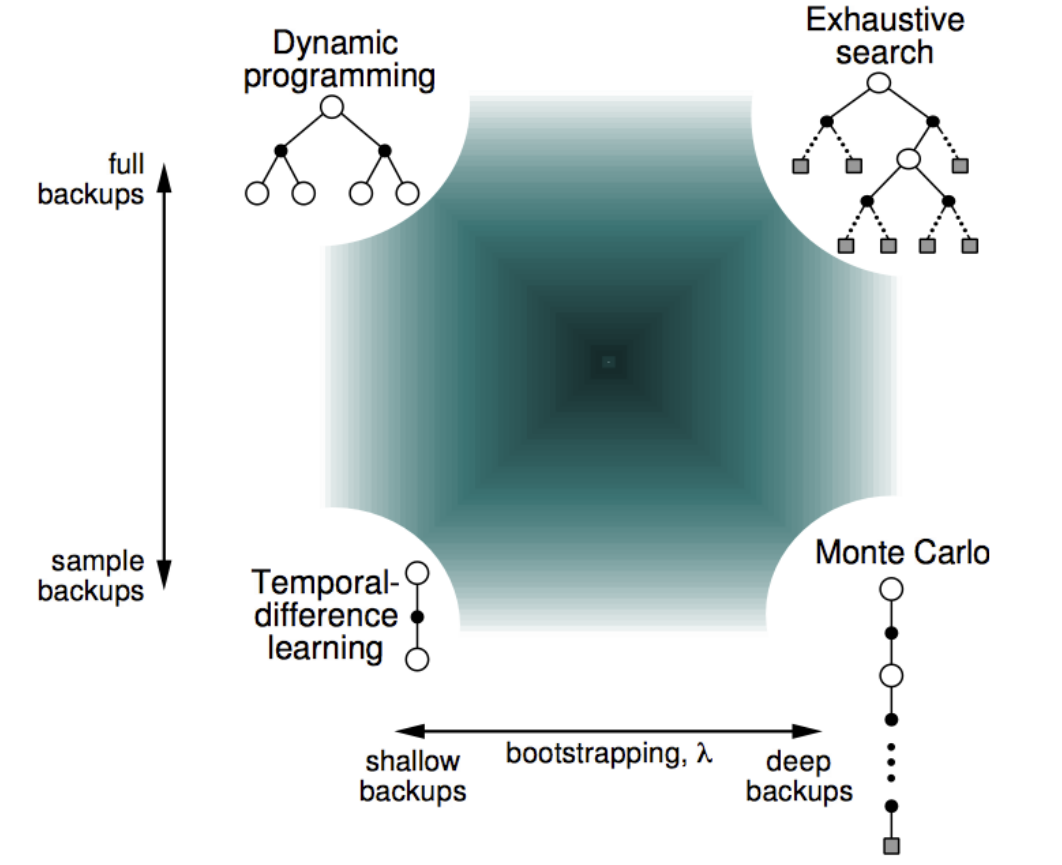
\includegraphics[width=0.75\textwidth]{figures/uni-rl.png}
    \caption{Unified View of Reinforcement Learning}
    \label{fig:uni-rl}
\end{figure}

\subsection{TD(\(\lambda \))}
TD(\(\lambda \)) is a family of methods that interpolate between MC and TD.
\subsubsection{\(n\)-step Prediction}
Let the TD target look \(n\) steps into the future as shown in \autoref{fig:td-n}.
\begin{figure}[H]
    \centering
    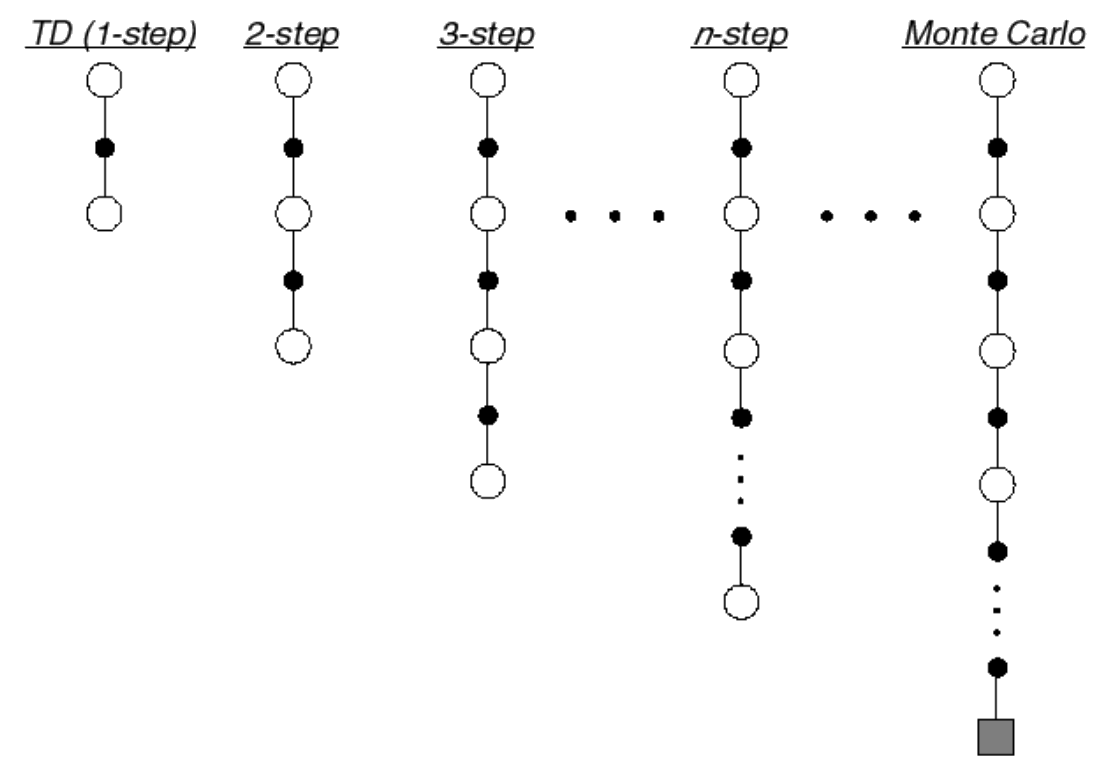
\includegraphics[width=0.75\textwidth]{figures/td-n.png}
    \caption{\(n\)-step Prediction of TD(\(\lambda \))}
    \label{fig:td-n}
\end{figure}
Consider the following \(n\) step returns for \(n = 1, 2, \dots \infty \):
\[
    \begin{aligned}
        n & = 1 \implies  G_t^{(1)} = R_{t+1} + \gamma V(S_{t+1}) &&\qquad \text{TD(0)} \\
        n & = 2 \implies  G_t^{(2)} = R_{t+1} + \gamma R_{t+2} + \gamma^2 V(S_{t+2}) \\
        \vdots \\
        n & = \infty \implies  G_t^{(\infty)} = R_{t+1} + \gamma R_{t+2} + \dots + \gamma^{T-1}R_T
        &&\qquad \text{MC} \\
    \end{aligned}
\]
Define the \(n\)-step return as,
\[
    G_t^{(n)} = R_{t+1} + \gamma R_{t+2} + \dots + \gamma^{n-1}R_{t+n} + \gamma^n V(S_{t+n})
\]
Thus, the \(n\)-step TD update is given as,
\[
    V(S_t) \leftarrow V(S_t) + \alpha\left( 
        G_t^{(n)} - V(S_t)
     \right)
\]

\subsubsection*{Average of \(n\)-step Returns}
We can also take the average of the \(n\)-step returns over different values of \(n\).
As example, we can take the average of the 2-step and 4step returns as,
\[
    \frac{1}{2}G^{(2)} + \frac{1}{2}G^{(4)}
\]
This allows us to combine information from two different time steps. There is much better
and efficient way to combine information from different time steps, using geometrically
decaying weights for the \(n\)-step returns. This is called as the \(\lambda\)-return.

\subsubsection{Forward View of TD(\(\lambda \))}

The tree backup of TD(\(\lambda \)) is shown in \autoref{fig:td-lambda}.
\begin{figure}[H]
    \centering
    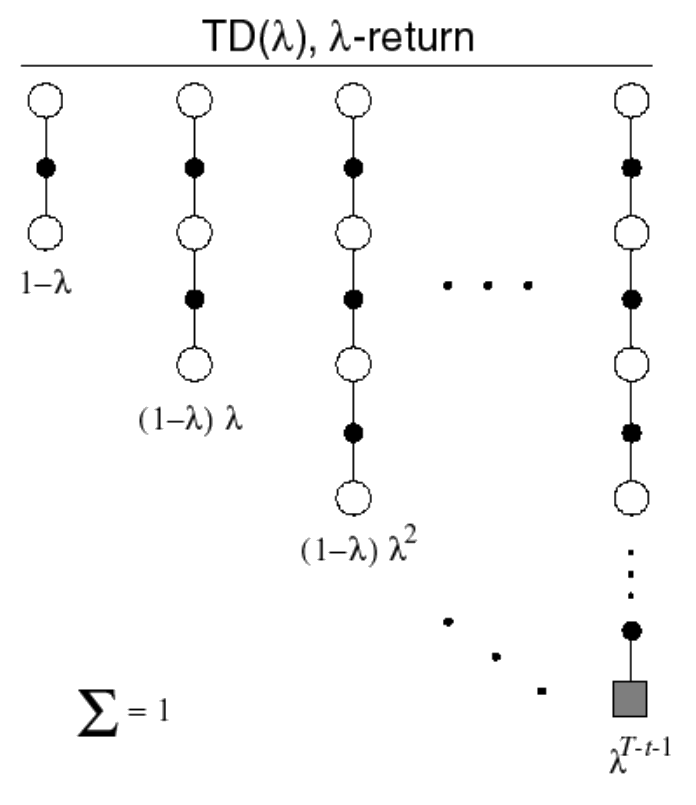
\includegraphics[width=0.5\textwidth]{figures/l-return.png}
    \caption{Tree Backup of TD(\(\lambda \))}
    \label{fig:td-lambda}
\end{figure}
The \(\lambda\)-return \(G_t^\lambda \) combines all the \(n\)-step returns with 
geometrically decaying weights. Using the weights \((1-\lambda)\lambda^{n-1}\), the return
\(G_t^\lambda \) is given as,
\[
    G_t^\lambda = (1-\lambda)\sum_{n=1}^{\infty}\lambda^{n-1}G_t^{(n)}
\]
where the factor \((1-\lambda)\) is used to normalize the weights. Thus, the forward view
of TD(\(\lambda \)) is given as,
\[
    V(S_t) \leftarrow V(S_t) + \alpha\left( 
        G_t^\lambda - V(S_t)
     \right)
\]
The weighting function is shown in \autoref{fig:lambda-weights}.
\begin{figure}[H]
    \centering
    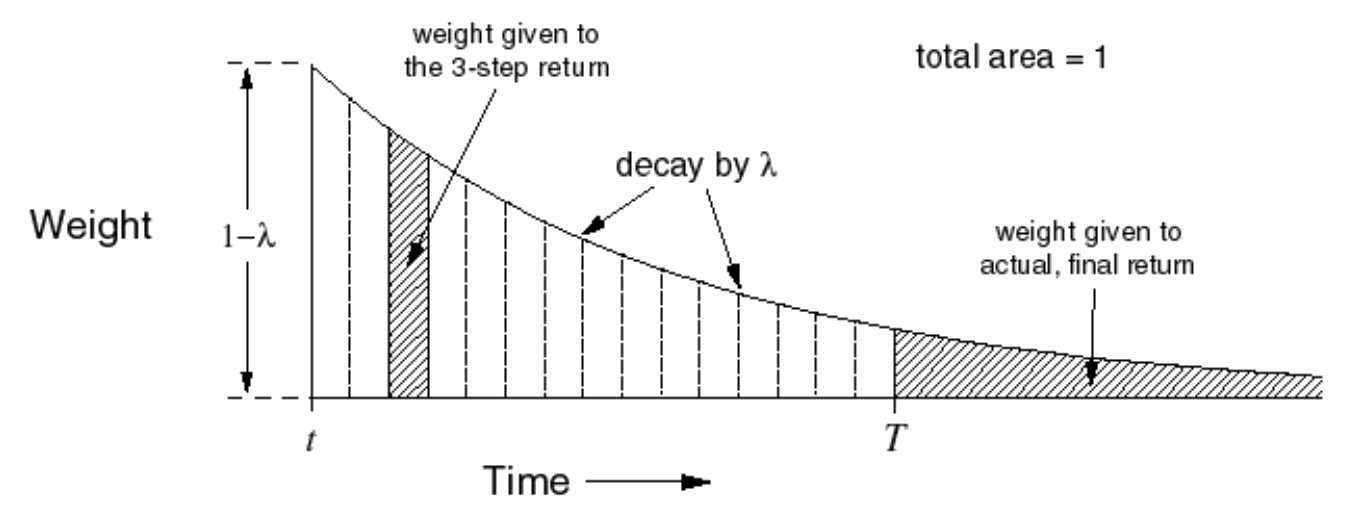
\includegraphics[width=0.9\textwidth]{figures/l-weights.png}
    \caption{Weights of TD(\(\lambda \) Weighting Function)}
    \label{fig:lambda-weights}
\end{figure}

\subsubsection{Eligibility Traces}
The eligibility trace \(E_t(s)\) is a measure of the credit assignment problem. 
Consist of the following two components:
\begin{itemize}
    \item \emph{Frequency heuristics}: assign the credit of reward or the bellamn error to
    the states that are visited more frequently.
    \item \emph{Recency heuristics}: assign the credit of reward or the bellamn error to
    the states that are visited more recently.
\end{itemize}
Eligibility traces combine both the frequency and recency heuristics, and is defined as,
\[
    \begin{aligned}
        E_0(s) &= 0 \\
        E_t(s) &= \gamma\lambda E_{t-1}(s) + \bm{1}(S_t = s)      
    \end{aligned}
\]
Thus, when we see some Bellman error or reward, we update the value function in the proportion
of the eligibility trace. 


\subsubsection{Backward View of TD(\(\lambda \))}
The algorithm for the backward view of TD(\(\lambda \)) is roughly as follows:
\begin{itemize}
    \item Keep an eligibility trace for every state \(s\)
    \item Update value \(V(s)\) for all states \(s\) visited in the episode, 
    in proportion to the TD-error \(\delta_t\) and the eligibility trace \(E_t(s)\).
    \[
        \begin{aligned}
            \delta _t &= R_{t+1} + \gamma V(S_{t+1}) - V(S_t) \\
            V(s) &\leftarrow V(s) + \alpha\delta_t E_t(s) \quad \forall s \in S_t
        \end{aligned}
    \] 
\end{itemize}
Intuitively the TD-error is being broadcasted into the past, and thus the value function is being
updated in the proportion of the eligibility trace and the TD-error. 

\subsubsection*{TD(\(\lambda \)) and TD(0)}
When \(\lambda = 0\), only the current state is being updated:
\[
    \begin{aligned}
        E_t(s) &= \bm{1}(S_t = s) \\
        V(s) &\leftarrow V(s) + \alpha\delta_t E_t(s) \quad \forall s \in S_t \\
        V(S_t) &\leftarrow V(S_t) + \alpha\delta_t
    \end{aligned}  
\]
which is equivalent to the TD(0) update.

\subsubsection*{TD(\(\lambda \)) and MC}
When \(\lambda = 1\), the credit is deferred until the end of the episode. Consider the 
case of episodic environment with offline update, then the total update for TD(1) is the same
as the total update for MC methods.
\begin{note}
    DID NOT UNDERSTAND THIS PART.
\end{note}